
\documentclass[11pt]{article}
%Gummi|065|=)
\title{\textbf{Projet Programmation imperative L2}\\ Morpion Solitaire}
\author{Guillaume Magniadas\\
		Tayebi Said Mahdi
		}
\date{}
\usepackage{graphicx}
\usepackage{listings}
\begin{document}

\maketitle
\begin{figure}[htp]
\centering
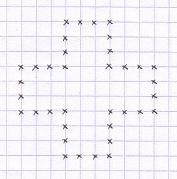
\includegraphics[scale=1.00]{index.jpg}
\caption{Morpion solitaire}

\label{}
\end{figure}

\newpage
\tableofcontents
\newpage

	\section{Introduction}
	\subsection{Morpion solitaire }


Le morpion solitaire est un jeu se jouant seul  qui malgrès son inspiration du morpion en demeure très différent. Le but ici est de réaliser un maximum de segment en partant d'une figure en forme de croix grecque. A chaque coup le joueur pose un nouveau point sur la grille de jeu de manière a former un segment de 5 points. Détail important, chaque segment ne peut avoir qu'un seul point en commun. Les points sont considéré comme alligné aussi bien a la vertical, l'horizontal et en diagonale.


\begin{figure}[htp]
\centering
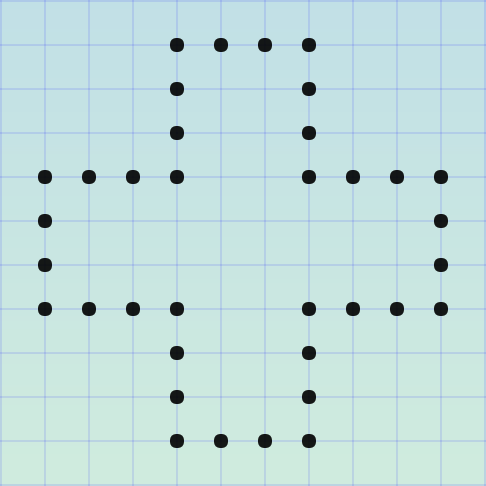
\includegraphics[scale=1.00]{croix_vide.png}
\caption{Croix greque}

\label{}
\end{figure}
\begin{figure}[htp]
\centering
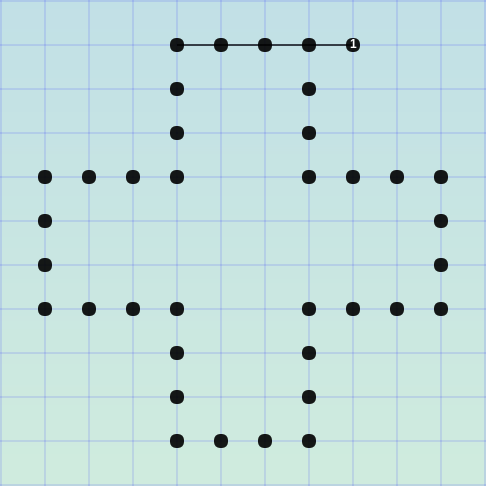
\includegraphics[scale=1.00]{Exemple_segment1.png}
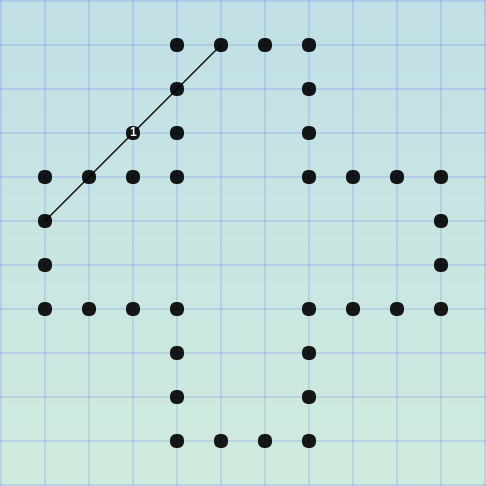
\includegraphics[scale=1.00]{Exemple_segment2.png}
\caption{Exemples de Coups possibles}
\label{}
\end{figure}
	\subsection {But du Projet}
		Sur ce projet notre but etait de realiser un programme capable d'obtenir le meilleur score possible et ce de maniere optimal en vue des possibilitées quasi infini du jeu.
	\subsection{Objectif}
Pour pouvoir atteindre ce but nous avions plusieurs objectif, premierement, introduire les regles permetant a partir d'un certaine etat connaitre tous les coups possible, puis de verifie si un ce segment ne croisera pas un autre segment .
\\
La deuxieme etape etait de pouvoir generer une liste de coups jouable a partir de n'importe quel etat de la grille de jeu.
\\
Et dernierement, creer une intélligence artifficiel pouvant a partir de n'importe quel (position mais surtout la position inital), trouver le plus grand score possible de maniere optimal.\\
	\subsection {Complexité du jeu}
	\subsubsection{Premier problème}
	Bien que qu'au premier abord les deux premier objectifs peuvent sembler assez simple, ils cachent des petits détail complexe, par rapport a un autre jeu possedant le même style de grille tel que le morpion  ou encore un puissance 4, un point (C'est a dire une case de coordonée X et Y) peu avoir plusieur coup jouable. En effet, un point ayant par exemple 4 points a sa gauche ainsi que 4 autres a sa droite n'aura pas 1 mais 5 choix, on se retrouve a avoir a plusieurs choix de creation de segment ce qui n'ai pas forcement le cas pour un autre jeu.
\begin{figure}[htp]
\centering
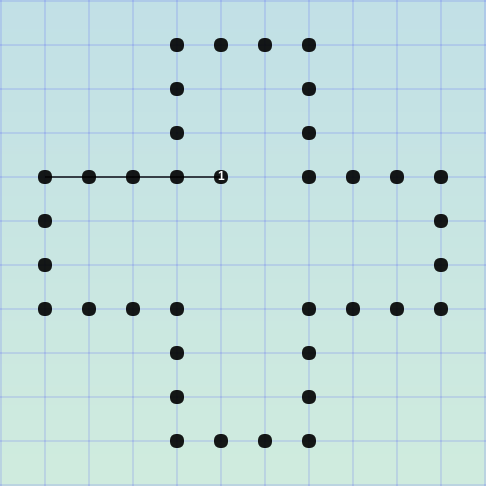
\includegraphics[scale=1.00]{position1.png}
\caption{Position initiale}
\label{}
\end{figure}
\begin{figure}[htp]
\centering
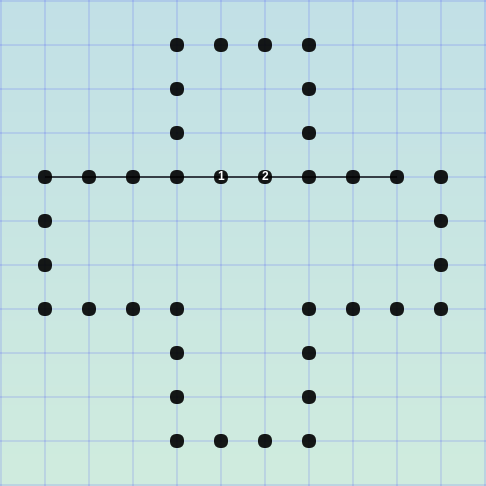
\includegraphics[scale=1.00]{position2_1.png}
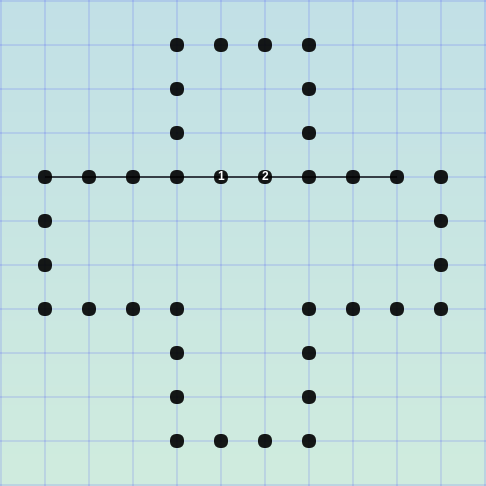
\includegraphics[scale=1.00]{position2_1.png}
\caption{Deux enfants possible différents}
\label{}
\end{figure}
	\subsubsection{Second problème}
Ensuite concernant l'inteligence artificiel, le morpion solitaire possede un graphe particulierement grand , rien que pour les 3 premiere profondeur le nombre de noeud dépasse 12.000 et pour les 8 premiere le nombre de noeud dépasse 29 Milliards (En prenant en compte les noeuds similaire). Ce probleme rend compliqué le parcours de graphe sans heuristique. Et par chance, il n'y a pas d'heuristique intéréssante connue, rendant la recherche d'une bonne ia fastidieuse.

		\section{Nos  structure}
		\subsection{point}
		Pour definir un point dans le tableau nous avons defini:\newline
		\begin{lstlisting}
struct point{
	int x;
	int y;
	int val;
	int possible;
	int totalligne;
	int totalcolonne;
	int totaldiagocroi;
	int totaldiagode;
	int total;
};
typedef struct point point;

\end{lstlisting}
		Deux entiers x et y pour definir leur position dans le tableau.\newline
		Possible represente le sens des coups possible, elle peut prendre des valeur entre 0 et 15, 0 indiquand que le point ne peut generer aucun segment, 15 que le point peut generer au moins 1 segment par sens.\\
		la famille des total represente le nombre de segment que l'on peut creer dans chaque sens et en tout.\\
		\subsection{Segement}
				\begin{lstlisting}
				
struct segment{
	point numero[5];
};
typedef struct segment segment;

\end{lstlisting}
Un segment est composé de 5 points.\\
(Dans le suite de ce rapport nous utiliserons souvent un tableau de segment nommé hist et utilisant la premiere case (hist[0].numero[0].val) comme indicateur sur le nombre d'éléments de ce tableau, comme aurait pus le faire une structure vecteur.)\\
\subsection{Coup jouable}
\begin{lstlisting}

struct coup_jouable{
	point courant;
	int sens;
	int nbsegment;
};
typedef struct position position;

\end{lstlisting}
Un coup jouable est un point ainsi qu'un sens et qu'un numero de segment.\\
Sens vaut une valeur entre 1, 2, 4 ou 8 représentant chacun un sens possible.\\
Nbsegment vaut le numero du segment possible dans le sens associé (Utile quand plusieurs segment sont possible sur le même sens).\\
Plus de detail sur les valeur de sens et de nbsegment dans la section mode d'emploie.\\
(Dans la suite de ce rapport nous utiliserons souvent un tableau de coup-jouable nommé listecoup et utilisant la premiere case (listecoup[0].sens) comme indicateur sur le nombre d'éléments de ce tableau, comme aurait pus le faire une structure vecteur.)\\
\subsection{Position}
				\begin{lstlisting}
struct position{
	int visits;
	segment *hist;
	int nbenfants;
	struct position* *enfants;
	int *visitchem;
	int *scorechem;
	int toutvisit;
	int terminal;
};
typedef struct position position;

\end{lstlisting}
Une structure contenant des informations sur un noeud,\\visits qui contient son le nombre de fois qu'un noeud a été visité,\\hist qui contient le tableau de segment correspondant a l'historique des coups joué,\\nbenfants qui contient le nombre d'enfants que possède le noeud,\\enfants qui est un tableau de pointeur de position contenant les adresses de ses enfants,\\visitchem et scorechem qui sont des tableau d'int,\\contenant le score et le nombre de visites de ses enfant (On utilise ces tableaux plutot que les valeurs stocké dans les enfants pour les cas d'enfant possedant d'autre parents),\\toutvisit est un simple flag qui indique si tout les enfants ont été exploré au moins une fois on non\\et terminal est un autre flag qui indique si la position est terminal (C'est a dire que son nombre de coups jouable possible vaut 0).\\
	\begin{lstlisting}
struct vecpos{
	int nb;
	struct position* *pointeur;
};
typedef struct vecpos vecpos;

\end{lstlisting}
Il sagit d'un vecteur de pointeur de position, il stockera tout les noeuds que l'ia explorera.\\
\subsection{Autre}
	\begin{lstlisting}

struct vecint{
	int nb;
	int *v;
};

\end{lstlisting}
Il sagit d'un vecteur d'int, tout simplement.\\
	\begin{lstlisting}
struct best{
	int retro;
	int score;
	int i;
};
typedef struct best best;

\end{lstlisting}
Sert à la fonction selection pour lui permettre de renvoyer la position du prochain enfant (La variable i), le score qu'il a obtenue (la variable score) et si un noeud à été créée et dans ce cas là lui indiquer qu'il faut revenir a la base de l'arbre (la variable retro).\\

\section{Nos fonction} 
Seul les fonction principales seront abordé, 
nous aurons deux sous-categories la premier sera lié au jeu du morpion solitaire en lui même et la deuxieme au sujet de l'IA et de son developpement.\\
\subsection{jouer au morpion solitaire}
\subsubsection{Jouable}
	\begin{lstlisting}
void jouable(point tab[TAILLE][TAILLE],int x,int y){
	int i, compte1, compte2;
	int lignes, colones, diagocroi, diagode;
	tab[x][y].possible=0;
	tab[x][y].total=0;
	lignes=0;
	colones=0;
	diagocroi=0;
	diagode=0;
	if(tab[x][y].val!=0){
		return;
	}
	else if(x+1>=TAILLE || y+1>=TAILLE|| x-1<0 || y-1<0 ||
	(tab[x+1][y].val==0 && tab[x-1][y].val==0 &&
	tab[x][y+1].val==0 && tab[x][y-1].val==0 &&
	tab[x+1][y+1].val==0 && tab[x-1][y-1].val==0 &&
	tab[x+1][y-1].val==0 && tab[x-1][y+1].val==0)){
		return;
	}
	else{
	
		for (i = 1, compte1=0, compte2=0; i < 5; ++i){ 
		  	if(tab[x+i][y].val==1 && compte1==i-1){
		  		compte1++;
		  	}
		  	if(tab[x-i][y].val==1 && compte2==i-1){
		  		compte2++;	
		  	}
		}
		if(compte1+compte2>3){
			lignes=1;
			tab[x][y].totalligne=compte1+compte2-3;
		}
		
		for (i = 1, compte1=0, compte2=0; i < 5; ++i){
			if(tab[x][y+i].val==1 && compte1==i-1){
				compte1++;
			}
			if(tab[x][y-i].val==1 && compte2==i-1){
				compte2++;
			}
		}
		if(compte1+compte2>3){
			colones=2;
			tab[x][y].totalcolonne=compte1+compte2-3;
		}

		for (i = 1, compte1=0, compte2=0; i < 5; ++i){
			if(tab[x+i][y+i].val==1 && compte1==i-1){
				compte1++;
			}
			if(tab[x-i][y-i].val==1 && compte2==i-1){
				compte2++;
			}
		}
		if(compte1+compte2>3){
			diagocroi=4;
			tab[x][y].totaldiagocroi=compte1+compte2-3;
		}

		for (i = 1, compte1=0, compte2=0; i < 5; ++i){
			if(tab[x+i][y-i].val==1 && compte1==i-1){
				compte1++;
			}
			if(tab[x-i][y+i].val==1 && compte2==i-1){
				compte2++;
			}
		}
		if(compte1+compte2>3){
			diagode=8;
			tab[x][y].totaldiagode=compte1+compte2-3;
		}
		
		tab[x][y].possible=lignes + colones + diagocroi + diagode;
		tab[x][y].total=tab[x][y].totalligne +
		tab[x][y].totalcolonne + tab[x][y].totaldiagocroi
		+ tab[x][y].totaldiagode;
	}
}

\end{lstlisting}
Cette fonction jouable va pour un point donné et un etat (le tableau de points) remplire toute les informations a son sujet dans le tableau de points. On regarde d'abords pour le nombre de points sur la même ligne sans interuptions, puis si il y en a plus de 3, on ajoute ce nombre de points - 3 à totalligne et on met 1 à lignes, et on répète cette opération pour les 3 autre sens pour seul différence le nom des variable (Au lieu de mettre 1 comme pour lignes, on met 2 pour colonnes, 4 pour diagocroi et 8 pour diagode).
A la fin on regle total sur la somme de tout les total de sens et possible sur la somme de lignes, colonnes, diagocroi et diagode.\\
\subsubsection{Historique}
\begin{lstlisting}
int historique(segment *hist,segment coup){
   	int cpt, i, j, k;
   	for (i = 1,cpt=0; i < MAXSEGMENT;++i,cpt=0){
   		if(hist[0].numero[0].val<i){
   	      	return 0;
   		}
   	    for(j = 0; j < 5; ++j){
   	    	for (k = 0; k < 5; ++k){
   	        	if(hist[i].numero[j].x==coup.numero[k].x &&
   	        	hist[i].numero[j].y==coup.numero[k].y){
   	           		++cpt;
   	           	}
   	           	if(cpt>1){
   	           		return 1;
   	           	}
   	      	}
   		}
   	}
   	printf("TAILLE HISTORIQUE DEPASSE\n");
   	return 0;
}
\end{lstlisting}
Cette fonction historique permet de savoir si un segment peut être joué par rapport a un tableau de segment donnée (Un segment peut être joué si il a au maximum un point en commun avec tout les autres segment déjà posé). Elle retourne 1 si il a plus de deux points commun avec un autre segment et 0 sinon.\\
\subsubsection{Coupjouable}
\begin{lstlisting}
void coupjouable(point tab[TAILLE][TAILLE],
coup_jouable listecoup[MAXLISTECOUP],segment *hist){
int i, j, k, possitest;
segment new;
listecoup[0].sens=0;
for (i = 0; i < TAILLE; ++i){
for(j=0;j<TAILLE;j++){
possitest=tab[j][i].possible;
if(possitest>0 && tab[j][i].val==0){
if(possitest & 1){
	for(k=0;k<tab[j][i].totalligne;++k){
		new=jouerpoint(tab,j,i,1,k);
		if(!historique(hist,new)){
			++listecoup[0].sens;
			listecoup[listecoup[0].sens].courant=tab[j][i];
			listecoup[listecoup[0].sens].sens=1;
			listecoup[listecoup[0].sens].nbsegment=k;
		}
	}
}
if(possitest & 2){
	for(k=0;k<tab[j][i].totalcolonne;++k){
		new=jouerpoint(tab,j,i,2,k);
		if(!historique(hist,new)){
			++listecoup[0].sens;
			listecoup[listecoup[0].sens].courant=tab[j][i];
			listecoup[listecoup[0].sens].sens=2;
			listecoup[listecoup[0].sens].nbsegment=k;
		}
	}
}
if(possitest & 4){
	for(k=0;k<tab[j][i].totaldiagocroi;++k){
		new=jouerpoint(tab,j,i,4,k);
		if(!historique(hist,new)){
			++listecoup[0].sens;
			listecoup[listecoup[0].sens].courant=tab[j][i];
			listecoup[listecoup[0].sens].sens=4;
			listecoup[listecoup[0].sens].nbsegment=k;
		}
	}
}
if(possitest & 8){
	for(k=0;k<tab[j][i].totaldiagode;++k){
		new=jouerpoint(tab,j,i,8,k);
		if(!historique(hist,new)){
			++listecoup[0].sens;
			listecoup[listecoup[0].sens].courant=tab[j][i];
			listecoup[listecoup[0].sens].sens=8;
			listecoup[listecoup[0].sens].nbsegment=k;
		}
	}
}
}
}
}
}

\end{lstlisting}
Cette fonction coupjouable est une des fonctions centrale de notre programme, elle va pour chaque point tester les segments possibles dans chacun des sens si leur valeur de possible correspond.\\L'interet de sauvegarder le nombre de segments possible dans chaque sens se retrouve ici, en faisant une boucle partant de 0 jusqu'au maximum de segment dans le sens, on va tester tout les segments possible de ce dernier (Chaque sens possède une fonction qui va remplir le segment new selon le sens actuel et le numéro du segment), puis on verifie si ce segment n'est pas en contact avec plus d'un point d'un autre segment de notre hist en passant ce nouveau segment et hist à la fonction historique décrite plus haut.\\Dans le cas ou historique renvoie 0, on ajoute le point courant, les informations sur son sens et son numero de segment dans le tableau de coup jouable.\\
\\
\\
\\
\subsection{Un peu d'IA}
\begin{lstlisting}

int ia(point tab[TAILLE][TAILLE],coup_jouable *listecoup,
segment *hist, vecint *cheminfinal, int objectif){
	int nb, maxxx, choix, compteur, scorestart;
	best final;
	point copy[TAILLE][TAILLE];
	segment *copyhist;
	position *actuel, *depart;
	vecpos listepos;
	vecint descente;

	descente=remplirvecint(MAXSEGMENT);
	listepos=remplirvec(MAXPOSITION);
	copyhist=malloc(MAXSEGMENT*sizeof(segment));
	copy_tab(tab,copy);
	copy_hist(hist,copyhist);

	coupjouable(copy,listecoup,copyhist);
	nb=listecoup[0].sens;

	listepos.pointeur[0]=malloc(sizeof(position));
	remplirPosition(nb,listepos.pointeur[0],hist);
	++listepos.nb;

	depart=listepos.pointeur[0];
	actuel=depart;
	depart->visits=1;

	scorestart=actuel->hist[0].numero[0].val;
	maxxx=0;
	compteur=0;

	for(;;){
	for(final=selection(listecoup,&listepos,actuel,copy);
	!actuel->terminal;final=
	selection(listecoup,&listepos,actuel,copy)){
		descente.v[descente.nb]=final.i;
		++descente.nb;
		if(final.retro){
			ajouterscorechemin(depart,descente,final.score);
			final.retro=0;
			break;
		}
		copy_hist(actuel->hist,copyhist);
		jouersurlistecoup(copy,listecoup,copyhist,final.i);
		actuel=actuel->enfants[final.i];
		coupjouable(copy,listecoup,actuel->hist);
	}
	if(maxxx<descente.nb+scorestart){
		compteur=0;
		maxxx=descente.nb+scorestart;
		copy_vecint(descente,cheminfinal);
		if(maxxx>=objectif){
			printf("Score de %d obtenue.
			Voulez vous continuer ? [1/0] : ",maxxx);
			scanf("%d",&choix);
			if(choix==0){
				liberertout(copyhist,&descente,&listepos);
				return maxxx;
			}
			else if(choix==1){
				++objectif;
			}
		}
	}
	++compteur;
	if(compteur>5000){
		printf("Voulez vous toujours continuer ? [1/0] : ");
		scanf("%d",&choix);
		if(choix==0){
			liberertout(copyhist,&descente,&listepos);
			return maxxx;
		}
		else if(choix==1){
			compteur=0;
		}
	}
	copy_tab(tab,copy);
	actuel=depart;
	descente.nb=0;
	coupjouable(copy,listecoup,actuel->hist);
	}
}

\end{lstlisting}
Voici la fonction principale de l'intelligence artificielle de notre programme.\\Nous allons résumer brievement son fonctionnement, elle est inspiré de l'algorithme "Recherche arborescente Monte-Carlo" (Un algorithme de recherche).\\L'ia est divisé en plusieurs étapes.
\\
\\La Selection :\\
- Si toutes les actions ont déjà été testées au moins une fois, elle calcule le score pour chacune et choisit la meilleure et continues la sélection dans la position suivante.\\- Si il y a au moins une action qui a été testée 0 fois, elle en choisis une et passe à l’expansion.\\
\\
L'Expansion :\\
- Ajoute une nouvelle position dans l’arbre qui correspond à la nouvelle action testée et vérifie si il ne sagit pas d'une position déjà existante et si c'est le cas recupere le pointeur de la position déjà existante.
\\
\\La Simulation :\\
- Joue au hasard à partir de la nouvelle position jusqu’à la fin de la partie et remonte son score puis le stocke.\\- Si la nouvelle position est déjà une fin de partie, passe à la phase de rétro-propagation.
\\
\\La rétro-propagation :\\
- pour chaque noeud visités pendant la sélection et l'expansion, incrementes le nombre de visite du noeud de 1 et ajoute le score obtenu au cumul des scores.
\section{Répartition du travail}
\subsection{Mehdi}
j'ai fait les bases du programme pour pouvoir poser des pions (La fonction jouable),
j'ai travailler sur un brouillon de fonction qui nous permeter d'optimiser le programme mais qui s'est averé innutile en vue du temps que ca prenait ca nous faisait plus perdre du temps qu'en gagner, la fonction historique pour gerer les segments et creer segements,
reorganiser les fichiers de sorte a ce qu'ils soient correctment placé.
J'ai aussi travaillé sur une interface graphique mais qui fut abandonné etant donné que l'objectif de notre projet n'etait pas vraiment d'avoir un beau rendu mais de bon resultats.
\subsection{Guillaume}
De mon coté, je me suis surtout occupé de l'intelligence artificielle et de tout ce qui en découle c'est à dire de la création d'une structure permetant de lister précisement les coups possible pour faciliter le choix des coups par l'ia (et donc des fonctions pour créer des segments et tout ce qui utilise cette liste de coup pour jouer dessus, la lire ou l'actualiser), et bien sur les fonctions principales de l'ia (ia, selection, expansion et les fonctions utilisant le vecteur de positions).
\section{Mode d'emploi}
		Dès le lancement du programme, on vous demandera un score a atteindre (Nous conseillons de choisir 90 en tant que premier choix).\newline Apres cela la partie est lanceé. Si le programme atteind le score désiré on vous proposera soit de continuer, soit d'arreter, si vous continuez on augmente votre objectif de 1, sinon vous arretez l'exploration actuel, On vous demandera si vous souhaitez reprendre mais à une profondeur différente basé sur les meilleurs profondeur parcouru dans l'essaie précédent et quel est votre nouveau score objectif (Nous vous conseillons d'augment le meilleur score précédent de seulement 1 ou 2).\newline Si vous choisissez d'arreter le programme, un fichier contenant l'ensemble de la partie avec les position joué sera créé au même emplacement que l'executable du programme.\\Sur le fichier obtenue il est question de sens et de numéro de segment.\\Le sens correspond au sens du segment, il y a 4 sens possible : 1, 2, 4 et 8. 1 correspond au sens horizontal, 2 au sens vertical, 4 au sens diagonale croissante et 8 au sens diagonale décroissante.\\Le numéro de segment sert a savoir de quel segment l'on parle lorsqu'il y a plus de 1 segment possible sur un même sens pour un point. (A lire de gauche à droite, ou de bas en haut)
		
		\section{Exemple d'utilisation}
		Voici une copie d'écran comme exemple d'utilisation de notre programme :
		\begin{figure}[!h]
\centering
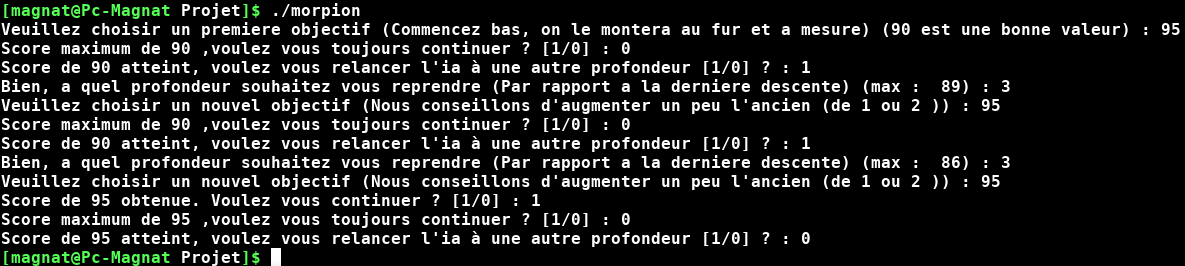
\includegraphics[scale=1.40]{screenderoulement.png}
\caption{Exemple}
\label{}
\end{figure}
\\A la suite de l'execution du programme, un fichier "Morpion\_solitaire\_score\_95.txt" à été généré contenant toutes les etapes (Les coups à jouer) de la croix grecque aux 95 coups :
\begin{figure}[!h]
\centering
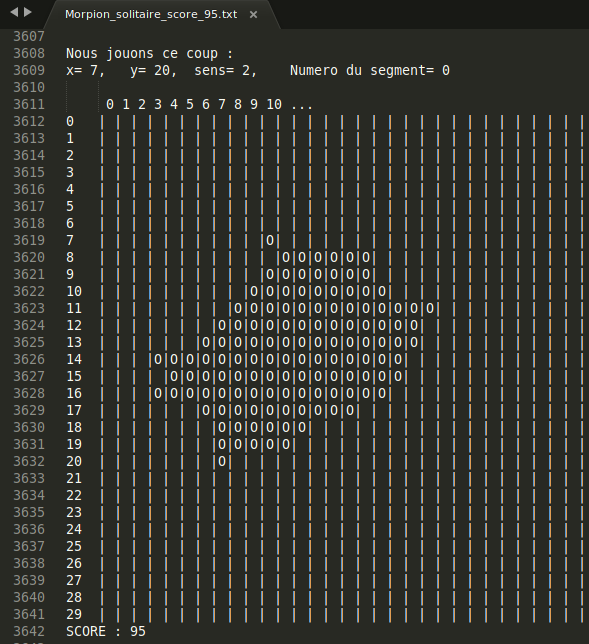
\includegraphics[scale=2.00]{exemple95.png}
\caption{Fichier généré}
\label{}
\end{figure}


		
		\section{Conclusion}
		Pour conclure sur ce sujet aussi passionant que le morpion solitaire, je voudrais souligner les difficultés epprouvé lors de la mise en place d'une IA capable de selectionner le bon chemin a suivre pour atteindre l'objectif souhaité, etant donné que le graphe augmente de maniere exponientiel, il n'y a pas d'algorithme specifique pour ce type de jeu, donc un grand effort d'abstaction fut neccessaire a la mise en place du jeu. Mais malgrès ces difficultés, ce sujet fut très intéréssant à penser et à developper.
		
\section{Remerciement}
Nous tenons à remercier Aline Hufschmitt (Doctorante en informatique à l'université Paris 8) pour l'aide précieuse qu'elle nous a fournis dans notre recherche d'une intelligence artificielle intéressante pour ce problème.

\section{Code source complet}
La suite de ce rapport contiendra le code source complet du programme y compris les fonctions et structure déjà présenté ci-dessus.
\subsection{Head.h}
\begin{verbatim}
#include <stdio.h>	
#include <stdlib.h>
#include <time.h>
#include <math.h>
#define TAILLE 30
#define MAXSEGMENT 200
#define MAXLISTECOUP 60

struct point{
	int x;
	int y;
	int val;
	int possible;
	int totalligne;
	int totalcolonne;
	int totaldiagocroi;
	int totaldiagode;
	int total;
};
typedef struct point point;

struct segment{
	point numero[5]; 
};
typedef struct segment segment;

struct coup_jouable{
	point courant;
	int sens;
	int nbsegment;
};
typedef struct coup_jouable coup_jouable;

struct position{
	int visits;
	segment *hist;
	int nbenfants;
	struct position* *enfants;
	int *visitchem;
	int *scorechem;
	int toutvisit;
	int terminal;
};
typedef struct position position;

struct vecpos{
	int nb;
	struct position* *pointeur;
};
typedef struct vecpos vecpos;

struct vecint{
	int nb;
	int *v;
};
typedef struct vecint vecint;

struct best{
	int retro;
	int score;
	int i;
};
typedef struct best best;

void affiche_point(point p);

void affiche_segment(segment s);

void affiche(point tab[TAILLE][TAILLE]);

void faffiche(point tab[TAILLE][TAILLE], FILE * f);

void sauvegarderdansfichier(int score, point tab[TAILLE][TAILLE],coup_jouable
*listecoup,segment *hist, vecint cheminfinal);

void jouable(point tab[TAILLE][TAILLE],int x,int y);

void coupjouable(point tab[TAILLE][TAILLE],coup_jouable
listecoup[MAXLISTECOUP],segment *hist);

void actualisepoint(point tab[TAILLE][TAILLE]);

int historique(segment *hist,segment coup);

segment jouerpoint(point tab[TAILLE][TAILLE], int x, int y, int sens, int nbsegment);
segment jouerpointcote(point tab[TAILLE][TAILLE], int x, int y, int nbsegment);
segment jouerpointhaut(point tab[TAILLE][TAILLE], int x, int y, int nbsegment);
segment jouerpointdiagocroi(point tab[TAILLE][TAILLE], int x, int y, int nbsegment);
segment jouerpointdiagode(point tab[TAILLE][TAILLE], int x, int y, int nbsegment);

void fill(point tab [TAILLE][TAILLE],int n);

void croix_greque(point tab[TAILLE][TAILLE],int n,int m);

void copy_tab(point tab[TAILLE][TAILLE],point copie[TAILLE][TAILLE]);

void copy_hist(segment *tab,segment *copy);

segment creersegment(point tab[TAILLE][TAILLE],int x1,int y1,int x2,int y2);

void jouersurlistecoup(point tab[TAILLE][TAILLE], coup_jouable
*listecoup, segment *hist, int quelcoup);

void jouerdescoups(point tab[TAILLE][TAILLE],coup_jouable *listecoup,
segment *hist, vecint chemin, int profondeur);

int choixaleatoire(int a, int b);

int jeualeatoire(point tab[TAILLE][TAILLE],coup_jouable *listecoup,segment *hist);

vecint remplirvecint(int reserve);

void copy_vecint(vecint original, vecint *copie);

vecpos remplirvec(int reserve);

void remplirPosition(int nbenfant, position* p, segment *hist);

void ajoueterdescente(vecint *descentefinal, vecint *chemin, int jusqua);

void ajouterscorechemin(position *depart, vecint chemin, int score);

void liberertout(segment* hist, vecint *descente, vecpos *listepos);

int ia(point tab[TAILLE][TAILLE],coup_jouable *listecoup,segment *hist,
vecint *cheminfinal, int objectif);

best selection(coup_jouable *listecoup, vecpos *listepos,
position *actuel, point tab[TAILLE][TAILLE]);

int expansion(point tab[TAILLE][TAILLE], coup_jouable *listecoup,
vecpos *listepos, position *actuel, int i);

int memehist(segment *hist, vecpos *listepos);

int memepos(segment *hist1, segment *hist2);

\end{verbatim}
Note : Tous les fichier incluront ce header.\\
\subsection{Affichage.c}
\begin{verbatim}
void affiche(point tab[TAILLE][TAILLE]){
	int i, j;
	printf("\t");
	for(i=0;i<11;++i){
		printf(" %d",i);
	}
	printf(" ...\n");
	for (i = 0; i < TAILLE; ++i){
		printf("%d\t|",i);
		for (j = 0; j < TAILLE; ++j){
	       	if(tab[j][i].val==0){
           		printf(" |");
	       	}
       		else{
       			printf("O|");
       		}
		}
		printf("\n");
	}
}

void faffiche(point tab[TAILLE][TAILLE], FILE * f){
	int i, j;
	fprintf(f,"\t");
	for(i=0;i<11;++i){
		fprintf(f," %d",i);
	}
	fprintf(f," ...\n");
	for (i = 0; i < TAILLE; ++i){
		fprintf(f,"%d\t|",i);
		for (j = 0; j < TAILLE; ++j){
	       	if(tab[j][i].val==0){
           		fprintf(f," |");
	       	}
       		else{
       			fprintf(f,"O|");
       		}
		}
		fprintf(f,"\n");
	}
}

void sauvegarderdansfichier(int score, point tab[TAILLE][TAILLE],
coup_jouable *listecoup,segment *hist, vecint cheminfinal){
	int nb, i;
	FILE * f;
	char nom[50];
	snprintf(nom, sizeof nom, "Morpion_solitaire_score_%d.txt", score);
	f = fopen(nom,"w+");
	nb=cheminfinal.nb;
	for(i=0;i<nb;++i){
		faffiche(tab,f);
		fprintf(f,"\nSCORE : %d\n",hist[0].numero[0].val);
		fprintf(f,"\n\nNous jouons ce coup : \n");
		fprintf(f,"x= %d, \ty= %d,\tsens= %d,\tNumero du segment= %d\n\n",
		listecoup[cheminfinal.v[i]+1].courant.x,listecoup[cheminfinal.v[i]+1].courant.y,
		listecoup[cheminfinal.v[i]+1].sens,listecoup[cheminfinal.v[i]+1].nbsegment);
		jouersurlistecoup(tab,listecoup,hist,cheminfinal.v[i]);
	}
	faffiche(tab,f);
	fprintf(f,"SCORE : %d\n",hist[0].numero[0].val);
}

\end{verbatim}
\subsection{Aleatoire.c}
\begin{verbatim}
int choixaleatoire(int a, int b){
	return rand()%(1+b-a) + a;
}

int jeualeatoire(point tab[TAILLE][TAILLE],coup_jouable *listecoup,segment *hist){
	int choix; //i;
	segment new;
	if(listecoup[0].sens==0){
		return hist[0].numero[0].val;
	}
	choix=choixaleatoire(1, listecoup[0].sens);
	new=jouerpoint(tab,listecoup[choix].courant.x,listecoup[choix].courant.y,listecoup[choix].sens,listecoup[choix].nbsegment);
	hist[1+hist[0].numero[0].val]=new;
	hist[0].numero[0].val+=1;
	tab[listecoup[choix].courant.x][listecoup[choix].courant.y].val=1;
	actualisepoint(tab);
	coupjouable(tab,listecoup,hist);
	return jeualeatoire(tab,listecoup,hist);
}

\end{verbatim}
\subsection{Deconmcts.c}
\begin{verbatim}
void liberertout(segment* hist, vecint *descente, vecpos *listepos){
	int i, nb;
	free(hist);
	free(descente->v);
	nb=listepos->nb;
	for(i=0;i<nb;++i){
		free(listepos->pointeur[i]->hist);
		free(listepos->pointeur[i]->enfants);
		free(listepos->pointeur[i]->visitchem);
		free(listepos->pointeur[i]->scorechem);
		free(listepos->pointeur[i]);
	}
	free(listepos->pointeur);
}

int ia(point tab[TAILLE][TAILLE],coup_jouable *listecoup,segment *hist,
vecint *cheminfinal, int objectif){
	int nb, maxxx, choix, compteur, scorestart;
	best final;
	point copy[TAILLE][TAILLE];
	segment *copyhist;
	position *actuel, *depart;
	vecpos listepos;
	vecint descente;

	descente=remplirvecint(MAXSEGMENT);
	listepos=remplirvec(MAXPOSITION);
	copyhist=malloc(MAXSEGMENT*sizeof(segment));
	copy_tab(tab,copy);
	copy_hist(hist,copyhist);

	coupjouable(copy,listecoup,copyhist);
	nb=listecoup[0].sens;

	listepos.pointeur[0]=malloc(sizeof(position));
	remplirPosition(nb,listepos.pointeur[0],hist);
	++listepos.nb;

	depart=listepos.pointeur[0];
	actuel=depart;
	depart->visits=1;

	scorestart=actuel->hist[0].numero[0].val;
	maxxx=0;
	compteur=0;

	for(;;){
		for(final=selection(listecoup,&listepos,actuel,copy);!actuel->terminal;
		final=selection(listecoup,&listepos,actuel,copy)){
			descente.v[descente.nb]=final.i;
			++descente.nb;
			if(final.retro){
				ajouterscorechemin(depart,descente,final.score);
				final.retro=0;
				break;
			}
			copy_hist(actuel->hist,copyhist);
			jouersurlistecoup(copy,listecoup,copyhist,final.i);
			actuel=actuel->enfants[final.i];
			coupjouable(copy,listecoup,actuel->hist);
		}
		if(maxxx<descente.nb+scorestart){
			compteur=0;
			maxxx=descente.nb+scorestart;
			copy_vecint(descente,cheminfinal);
			if(maxxx>=objectif){
				printf("Score de %d obtenue. Voulez vous continuer ? [1/0] : ",maxxx);
				scanf("%d",&choix);
				if(choix==0){
					liberertout(copyhist,&descente,&listepos);
					return maxxx;
				}
				else if(choix==1){
					++objectif;
				}
			}
		}
		++compteur;
		if(compteur>5000){
			printf("Voulez vous toujours continuer ? [1/0] : ");
			scanf("%d",&choix);
			if(choix==0){
				liberertout(copyhist,&descente,&listepos);
				return maxxx;
			}
			else if(choix==1){
				compteur=0;
			}
		}
		copy_tab(tab,copy);
		actuel=depart;
		descente.nb=0;
		coupjouable(copy,listecoup,actuel->hist);
	}
}

best selection(coup_jouable *listecoup, vecpos *listepos,
position *actuel, point tab[TAILLE][TAILLE]){
	int i, nb, save;
	best final;

	nb=listecoup[0].sens;
	final.score=0;
	final.i=-1;
	if(nb==0){
		actuel->terminal=1;
		return final;
	}
	else{
		if(!actuel->toutvisit){
			for(i=0;i<nb;++i){
				if(actuel->enfants[i]==NULL){
					if(expansion(tab,listecoup,listepos,actuel,i)){
						continue;
					}
					final.i=i;
					final.score=actuel->scorechem[i];
					final.retro=1;
					return final;
				}
			}
			actuel->toutvisit=1;
		}
		for(i=0;i<nb;++i){
			if(actuel->enfants[i]->terminal){
				continue;
			}
			save=actuel->scorechem[i]/actuel->visitchem[i]+1.4*
			sqrt(log(actuel->visits)/actuel->visitchem[i]);
			if(final.score<save){
				final.score=save;
				final.i=i;
			}
		}
		if(final.i==-1){

			actuel->terminal=1;
			return final;
		}
		return final;
	}
}

int expansion(point tab[TAILLE][TAILLE], coup_jouable *listecoup,
vecpos *listepos, position *actuel, int i){
	int save, where;
	point copy[TAILLE][TAILLE];
	segment *copyhist;
	copyhist=malloc(MAXSEGMENT*sizeof(segment));

	copy_tab(tab,copy);
	copy_hist(actuel->hist,copyhist);
	jouersurlistecoup(copy,listecoup,copyhist,i);
	where=memehist(copyhist,listepos);
	if(where){
		actuel->enfants[i]=listepos->pointeur[where];
		save=jeualeatoire(copy,listecoup,copyhist);
		actuel->scorechem[i]=save;
		actuel->visitchem[i]=1;

		coupjouable(tab,listecoup,actuel->hist);
		free(copyhist);
		return 1;
	}
	listepos->pointeur[listepos->nb]=malloc(sizeof(position));
	remplirPosition(listecoup[0].sens,listepos->pointeur[listepos->nb],copyhist);
	actuel->enfants[i]=listepos->pointeur[listepos->nb];
	++listepos->nb;

	save=jeualeatoire(copy,listecoup,copyhist);
	actuel->scorechem[i]=save;
	actuel->enfants[i]->visits=1;
	actuel->visitchem[i]=1;

	coupjouable(tab,listecoup,actuel->hist);
	free(copyhist);
	return 0;
}

\end{verbatim}
\subsection{Iastruct.c}
\begin{verbatim}
vecint remplirvecint(int reserve){
	int i;
	vecint v;
	v.nb=0;
	v.v=malloc(reserve*sizeof(int));
	for(i=0;i<reserve;++i){
		v.v[i]=0;
	}
	return v;
}

void copy_vecint(vecint original, vecint *copie){
	int i, nb;
	nb=original.nb;
	copie->nb=nb;
	for(i=0;i<nb;++i){
		copie->v[i]=original.v[i];
	}
}

vecpos remplirvec(int reserve){
	vecpos new;
	new.nb=0;
	new.pointeur=malloc(reserve*sizeof(position*));
	return new;
}

void remplirPosition(int nbenfant, position* p, segment *hist){
	int i;
	p->visits=0;
	p->hist=malloc(MAXSEGMENT*sizeof(segment));
	copy_hist(hist,p->hist);
	p->enfants=malloc(nbenfant*sizeof(position*));
	p->visitchem=malloc(nbenfant*sizeof(int));
	p->scorechem=malloc(nbenfant*sizeof(int));
	for(i=0;i<nbenfant;++i){
		p->enfants[i]=NULL;
		p->visitchem[i]=0;
		p->scorechem[i]=0;
	}
	p->toutvisit=0;
	p->terminal=0;
}

void ajoueterdescente(vecint *descentefinal, vecint *chemin, int jusqua){
	int nb, i;
	nb=descentefinal->nb;
	for(i=0;i<jusqua;++i){
		descentefinal->v[nb+i]=chemin->v[i];
	}
	descentefinal->nb+=jusqua;
}

void ajouterscorechemin(position *depart, vecint chemin, int score){
	int i, nb;
	position *actuel;
	actuel=depart;
	nb=chemin.nb;

	for(i=0;i<nb;++i){
		++actuel->visits;
		++actuel->visitchem[chemin.v[i]];
		actuel->scorechem[chemin.v[i]]+=score;
		actuel=actuel->enfants[chemin.v[i]];
	}
	++actuel->visits;
}

\end{verbatim}
\subsection{Jouable.c}
\begin{verbatim}
void jouable(point tab[TAILLE][TAILLE],int x,int y){
	int i, compte1, compte2;
	int lignes, colones, diagocroi, diagode;
	tab[x][y].possible=0;
	tab[x][y].total=0;
	lignes=0;
	colones=0;
	diagocroi=0;
	diagode=0;
	if(tab[x][y].val!=0){
		return;
	}
	else if(x+1>=TAILLE || y+1>=TAILLE|| x-1<0 || y-1<0 ||
	(tab[x+1][y].val==0 && tab[x-1][y].val==0 && tab[x][y+1].val==0 &&
	tab[x][y-1].val==0 && tab[x+1][y+1].val==0 && tab[x-1][y-1].val==0 &&
	tab[x+1][y-1].val==0 && tab[x-1][y+1].val==0)){
		return;
	}
	else{
		for (i = 1, compte1=0, compte2=0; i < 5; ++i){ 
		  	if(tab[x+i][y].val==1 && compte1==i-1){
		  		compte1++;
		  	}
		  	if(tab[x-i][y].val==1 && compte2==i-1){
		  		compte2++;	
		  	}
		}
		if(compte1+compte2>3){
			lignes=1;
			tab[x][y].totalligne=compte1+compte2-3;
		}
		for (i = 1, compte1=0, compte2=0; i < 5; ++i){
			if(tab[x][y+i].val==1 && compte1==i-1){
				compte1++;
			}
			if(tab[x][y-i].val==1 && compte2==i-1){
				compte2++;
			}
		}
		if(compte1+compte2>3){
			colones=2;
			tab[x][y].totalcolonne=compte1+compte2-3;
		}
		for (i = 1, compte1=0, compte2=0; i < 5; ++i){
			if(tab[x+i][y+i].val==1 && compte1==i-1){
				compte1++;
			}
			if(tab[x-i][y-i].val==1 && compte2==i-1){
				compte2++;
			}
		}
		if(compte1+compte2>3){
			diagocroi=4;
			tab[x][y].totaldiagocroi=compte1+compte2-3;
		}
		for (i = 1, compte1=0, compte2=0; i < 5; ++i){
			if(tab[x+i][y-i].val==1 && compte1==i-1){
				compte1++;
			}
			if(tab[x-i][y+i].val==1 && compte2==i-1){
				compte2++;
			}
		}
		if(compte1+compte2>3){
			diagode=8;
			tab[x][y].totaldiagode=compte1+compte2-3;
		}
		tab[x][y].possible=lignes+colones+diagocroi+diagode;
		tab[x][y].total=tab[x][y].totalligne+tab[x][y].totalcolonne+
		tab[x][y].totaldiagocroi+tab[x][y].totaldiagode;
	}
}

void coupjouable(point tab[TAILLE][TAILLE],coup_jouable
listecoup[MAXLISTECOUP],segment *hist){
	int i, j, k, possitest;
	segment new;
	listecoup[0].sens=0;
	for (i = 0; i < TAILLE; ++i){
		for(j=0;j<TAILLE;j++){
			possitest=tab[j][i].possible;
			if(possitest>0 && tab[j][i].val==0){
				if(possitest & 1){
					for(k=0;k<tab[j][i].totalligne;++k){
						new=jouerpoint(tab,j,i,1,k);
						if(!historique(hist,new)){
							++listecoup[0].sens;
							listecoup[listecoup[0].sens].courant=tab[j][i];
							listecoup[listecoup[0].sens].sens=1;
							listecoup[listecoup[0].sens].nbsegment=k;
						}
					}
				}
				if(possitest & 2){
					for(k=0;k<tab[j][i].totalcolonne;++k){
						new=jouerpoint(tab,j,i,2,k);
						if(!historique(hist,new)){
							++listecoup[0].sens;
							listecoup[listecoup[0].sens].courant=tab[j][i];
							listecoup[listecoup[0].sens].sens=2;
							listecoup[listecoup[0].sens].nbsegment=k;
						}
					}
				}
				if(possitest & 4){
					for(k=0;k<tab[j][i].totaldiagocroi;++k){
						new=jouerpoint(tab,j,i,4,k);
						if(!historique(hist,new)){
							++listecoup[0].sens;
							listecoup[listecoup[0].sens].courant=tab[j][i];
							listecoup[listecoup[0].sens].sens=4;
							listecoup[listecoup[0].sens].nbsegment=k;
						}
					}
				}
				if(possitest & 8){
					for(k=0;k<tab[j][i].totaldiagode;++k){
						new=jouerpoint(tab,j,i,8,k);
						if(!historique(hist,new)){
							++listecoup[0].sens;
							listecoup[listecoup[0].sens].courant=tab[j][i];
							listecoup[listecoup[0].sens].sens=8;
							listecoup[listecoup[0].sens].nbsegment=k;
						}
					}
				}
			}
		}
	}
}

void actualisepoint(point tab[TAILLE][TAILLE]){
	int i, j;
	for(i=0;i<TAILLE;++i){
		for(j=0;j<TAILLE;++j){
			jouable(tab,j,i);
		}
	}
}
\end{verbatim}
\subsection{Jouersens.c}
\begin{verbatim}
int historique(segment *hist,segment coup){
   	int cpt, i, j, k;
   	for (i = 1,cpt=0; i < MAXSEGMENT;++i,cpt=0){
   		if(hist[0].numero[0].val<i){
   	      	return 0;
   		}
   	    for(j = 0; j < 5; ++j){
   	    	for (k = 0; k < 5; ++k){
   	        	if(hist[i].numero[j].x==coup.numero[k].x &&
   	        	hist[i].numero[j].y==coup.numero[k].y){
   	           		++cpt;
   	           	}
   	           	if(cpt>1){
   	           		return 1;
   	           	}
   	      	}
   		}
   	}
   	printf("TAILLE HISTORIQUE DEPASSE\n");
   	return 0;
}

segment jouerpoint(point tab[TAILLE][TAILLE], int x,
int y, int sens, int nbsegment){
	if(sens & 1){
		return jouerpointcote(tab,x,y,nbsegment);
	}
	else if(sens & 2){
		return jouerpointhaut(tab,x,y,nbsegment);
	}
	else if(sens & 4){
		return jouerpointdiagocroi(tab,x,y,nbsegment);
	}
	else{
		return jouerpointdiagode(tab,x,y,nbsegment);
	}
}



segment jouerpointcote(point tab[TAILLE][TAILLE],int x, int y,int nbsegment){
	int i, compte1, compte2;
	for (i = 1, compte1=0, compte2=0; i < 5; ++i){ 
		if(tab[x+i][y].val==1 && compte1==i-1){
			compte1++;
		}
		if(tab[x-i][y].val==1 && compte2==i-1){
			compte2++;	
		}
	}
	return creersegment(tab, x-compte2+nbsegment, y, x+4-compte2+nbsegment, y);
}

segment jouerpointhaut(point tab[TAILLE][TAILLE],int x, int y,int nbsegment){
	int i, compte1, compte2;
	for (i = 1, compte1=0, compte2=0; i < 5; ++i){
		if(tab[x][y+i].val==1 && compte1==i-1){
			compte1++;
		}
		if(tab[x][y-i].val==1 && compte2==i-1){
			compte2++;
		}
	}
	return creersegment(tab, x, y+compte1-nbsegment, x, y-4+compte1-nbsegment);
}

segment jouerpointdiagocroi(point tab[TAILLE][TAILLE],int x, int y,int nbsegment){
	int i, compte1, compte2;
	for (i = 1, compte1=0, compte2=0; i < 5; ++i){
		if(tab[x+i][y+i].val==1 && compte1==i-1){
			compte1++;
		}
		if(tab[x-i][y-i].val==1 && compte2==i-1){
			compte2++;
		}
	}
	return creersegment(tab, x-compte2+nbsegment, y-compte2+nbsegment,
	x+4-compte2+nbsegment, y+4-compte2+nbsegment);
}

segment jouerpointdiagode(point tab[TAILLE][TAILLE],int x, int y,int nbsegment){	
	int i, compte1, compte2;
	for (i = 1, compte1=0, compte2=0; i < 5; ++i){
		if(tab[x+i][y-i].val==1 && compte1==i-1){
			compte1++;
		}
		if(tab[x-i][y+i].val==1 && compte2==i-1){
			compte2++;
		}
	}
	return creersegment(tab, x-compte2+nbsegment, y+compte2-nbsegment,
	x+4-compte2+nbsegment, y-4+compte2-nbsegment);
}
\end{verbatim}
\subsection{Main.c}
\begin{verbatim}
int main(int argc, char const *argv[]){
	int objectif, etat, nbdescente, fin, choix;
	point new[TAILLE][TAILLE], copy[TAILLE][TAILLE], fintab[TAILLE][TAILLE], seginfo;
	segment *hist, *copyhist, *finalhist;
	coup_jouable* listecoup;
	vecint descente, descentefinal;

	listecoup=malloc(sizeof(coup_jouable)*MAXLISTECOUP);
	finalhist=malloc(MAXSEGMENT*sizeof(segment));
	copyhist=malloc(MAXSEGMENT*sizeof(segment));
	hist=malloc(MAXSEGMENT*sizeof(segment));
	descente=remplirvecint(MAXSEGMENT);
	descentefinal=remplirvecint(MAXSEGMENT);

	seginfo.val=0;
	hist[0].numero[0]=seginfo;

	fill(new,0);
	croix_greque(new,6,6);
	actualisepoint(new);
	copy_tab(new,copy);
	copy_tab(new,fintab);
	copy_hist(hist,copyhist);
	copy_hist(hist,finalhist);

	coupjouable(copy,listecoup,copyhist);

	printf("Veuillez choisir un premiere objectif
	(Commencez bas, on le montera au fur et a mesure) (90 est une bonne valeur) : ");
	scanf("%d",&objectif);
	fin=1;
	for(;fin;){
		etat=ia(copy,listecoup,copyhist,&descente,objectif);
		while(1){
			printf("Score de %d atteint, voulez vous relancer l'ia
			à une autre profondeur [1/0] ? : ",etat);
			scanf("%d",&choix);
			if(choix==0){
				ajoueterdescente(&descentefinal,&descente,descente.nb);
				coupjouable(fintab,listecoup,finalhist);
				sauvegarderdansfichier(etat,fintab,listecoup,finalhist,descentefinal);
				fin=0;
				break;
			}
			else if(choix==1){
				printf("Bien, a quel profondeur souhaitez vous reprendre
				(Par rapport a la derniere descente) (max :  %d) : ", descente.nb-1);
				while(1){
					scanf("%d",&nbdescente);
					if(nbdescente>=descente.nb || nbdescente<0){
						printf("Veuillez choisir un nombre entre 0 et %d : ", descente.nb);
					}
					break;
				}
				ajoueterdescente(&descentefinal,&descente,nbdescente);
				coupjouable(new,listecoup,hist);
				jouerdescoups(new,listecoup,hist,descente,nbdescente);
				copy_tab(new,copy);
				copy_hist(hist,copyhist);
				printf("Veuillez choisir un nouvel objectif
				(Nous conseillons d'augmenter un peu l'ancien (de 1 ou 2 )) : ");
				scanf("%d",&objectif);
				break;
			}
			else{
				printf("Erreur de saisie\n");
				continue;
			}
		}
	}
	return 0;
}
\end{verbatim}
\subsection{Memehist.c}
\begin{verbatim}
int memehist(segment *hist, vecpos *listepos){
	int i, nb;
	nb=listepos->nb;
	for(i=0;i<nb;++i){
		if(listepos->pointeur[i]==NULL){
			continue;
		}
		if(memepos(hist,listepos->pointeur[i]->hist)){
			return i;
		}
	}
	return 0;
}

int memepos(segment *hist1, segment *hist2){
	int nb1, nb2, i, j, verif;
	nb1=hist1[0].numero[0].val;
	nb2=hist2[0].numero[0].val;
	if(nb1!=nb2){
		return 0;
	}
	for(i=1, verif=0;i<=nb2;++i){
		for(j=1;j<=nb1;++j){
			if(hist1[j].numero[0].x==hist2[i].numero[0].x &&
			hist1[j].numero[0].y == hist2[i].numero[0].y){
				if(hist1[j].numero[4].x==hist2[i].numero[4].x &&
				hist1[j].numero[4].y == hist2[i].numero[4].y){
					++verif;
					break;
				}
			}
		}
		if(!verif){
			return 0;
		}
	}
	if(verif==nb1){
		return 1;
	}
	return 0;
}
\end{verbatim}
\subsection{Remplissage.c}
\begin{verbatim}
void fill(point tab [TAILLE][TAILLE],int n)
{
	int i, j;
	for (i = 0; i < TAILLE; ++i){
	    for (j= 0; j < TAILLE; ++j){
			tab[j][i].x=j;
			tab[j][i].y=i;
			tab[j][i].val=n;
			tab[j][i].possible=0;
			tab[j][i].totalligne=0;
			tab[j][i].totalcolonne=0;
			tab[j][i].totaldiagocroi=0;
			tab[j][i].totaldiagode=0;
			tab[j][i].total=0;
		}
	}
}

void croix_greque(point tab[TAILLE][TAILLE],int n,int m){
	int i;
	for (i = 5; i < 9; ++i){
		tab[m+2][n+i].val=1;	
		tab[m+5][n+i-3].val=1;
		tab[m+5][n+i+3].val=1;
		tab[m+8][n+i-3].val=1;
		tab[m+8][n+i+3].val=1;
		tab[m+11][n+i].val=1;
	}
	for (i = 3; i < 5; ++i){
		tab[m+i][n+5].val=1;
		tab[m+i][n+8].val=1;
		tab[m+i+3][n+2].val=1;
		tab[m+i+3][n+11].val=1;
		tab[m+i+6][n+5].val=1;
		tab[m+i+6][n+8].val=1;
	}
}

void copy_tab(point tab[TAILLE][TAILLE],point copie[TAILLE][TAILLE]){
	int i, j;
	for (i = 0; i < TAILLE; ++i){
		for (j = 0; j < TAILLE; ++j){
			copie[i][j]=tab[i][j];

		}
	}
}

void copy_hist(segment *tab,segment *copy){
	int i;
	for(i=0;i<MAXSEGMENT;++i){
		copy[i]=tab[i];
	}
}

segment creersegment(point tab[TAILLE][TAILLE],int x1,int y1,int x2,int y2)
{
	int i, d, h;
	segment new;
	if(x1<x2){
		d=1;
	}
	else if(x1>x2){
		d=-1;
	}
	else{
		d=0;
	}
	if(y1<y2){
		h=1;
	}
	else if(y1>y2){
		h=-1;
	}
	else{
		h=0;
	}
	for (i = 0; i <5 ; ++i){
		new.numero[i]=tab[x1+d*i][y1+h*i];
	}
	return new;
}

void jouersurlistecoup(point tab[TAILLE][TAILLE], coup_jouable
*listecoup,segment *hist, int quelcoup){
	segment new;
	new=jouerpoint(tab,listecoup[quelcoup+1].courant.x,listecoup[quelcoup+1].courant.y,
	listecoup[quelcoup+1].sens,listecoup[quelcoup+1].nbsegment);
	hist[1+hist[0].numero[0].val]=new;
	hist[0].numero[0].val+=1;
	tab[listecoup[quelcoup+1].courant.x][listecoup[quelcoup+1].courant.y].val=1;
	actualisepoint(tab);
	coupjouable(tab,listecoup,hist);
}

void jouerdescoups(point tab[TAILLE][TAILLE],coup_jouable
*listecoup,segment *hist, vecint chemin, int profondeur){
	int i;
	for(i=0;i<profondeur;++i){
		jouersurlistecoup(tab,listecoup,hist,chemin.v[i]);
	}
}
\end{verbatim}
\subsection{Notre makefile}
\begin{verbatim}
CC=gcc
CFLAGS=-Wall
SRC=main.c jouable.c jouersens.c remplissage.c affichage.c
aleatoire.c iastruct.c deconmcts.c memehist.c

OBJ=main.o jouable.o jouersens.o remplissage.o affichage.o
aleatoire.o iastruct.o deconmcts.o memehist.o
HEAD=head.h 

morpion:    $(OBJ) $(HEAD)
	$(CC) $(OBJ) -o $@ -lm

%.o:	%.c
	$(CC) -c -O3 $< $(CFLAGS)

clean:
	rm *.o

cleanall:
	rm *.o morpion
\end{verbatim}
\end{document}































